%% ****** Start of file aiptemplate.tex ****** %
%%
%%   This file is part of the files in the distribution of AIP substyles for REVTeX4.
%%   Version 4.1 of 9 October 2009.
%%
%
% This is a template for producing documents for use with 
% the REVTEX 4.1 document class and the AIP substyles.
% 
% Copy this file to another name and then work on that file.
% That way, you always have this original template file to use.

%\documentclass[aip,graphicx]{revtex4-1}
%\documentclass[aip,reprint]{revtex4-1}

%\usepackage{graphicx}

%\draft % marks overfull lines with a black rule on the right
%\documentclass[pre,aps,floatfix,authordate1-4,twocolumn]{revtex4-1}
%\documentclass[pre,aps,floatfix,authordate1-4]{revtex4-1}

\documentclass[aip,jcp,twocolumn]{revtex4}
%\documentclass[aip,jcp]{revtex4}
%\documentclass{article}



%\documentclass[aps,prl,preprint,groupedaddress]{revtex4}

\usepackage{rotating} 
\usepackage{times}
\usepackage{graphicx}
\usepackage{setspace}
\usepackage{amsmath}
\usepackage{epstopdf}
\usepackage[obeyFinal]{easy-todo}
\usepackage{csquotes}
\usepackage{mhchem}
\usepackage{chemfig}

%\usepackage{markdown} 

\begin{document}

% Use the \preprint command to place your local institutional report number 
% on the title page in preprint mode.
% Multiple \preprint commands are allowed.
%\preprint{}

\title{Accurate binding of calcium to phospholipid bilayers by effective inclusion of electronic polarization} %Title of paper

% repeat the \author .. \affiliation  etc. as needed
% \email, \thanks, \homepage, \altaffiliation all apply to the current author.
% Explanatory text should go in the []'s, 
% actual e-mail address or url should go in the {}'s for \email and \homepage.
% Please use the appropriate macro for the type of information

% \affiliation command applies to all authors since the last \affiliation command. 
% The \affiliation command should follow the other information.

\author{Josef Melcr}
\author{Hector Martinez-Seara Monne}
\affiliation{Institute of Organic Chemistry and Biochemistry,
Academy of Sciences of the Czech Republic, 
Prague 6, Czech Republic}
\author{Pavel Jungwirth}
\affiliation{Institute of Organic Chemistry and Biochemistry,
Academy of Sciences of the Czech Republic, 
Prague 6, Czech Republic}
\affiliation{Department of Physics, Tampere University of Technology, P.O. Box 692, FI-33101
Tampere, Finland}

\author{O. H. Samuli Ollila}
\email[]{samuli.ollila@helsinki.fi}
%\homepage[]{Your web page}
\affiliation{Institute of Organic Chemistry and Biochemistry,
Academy of Sciences of the Czech Republic, 
Prague 6, Czech Republic}
\affiliation{Institute of Biotechnology, University of Helsinki}


% Collaboration name, if desired (requires use of superscriptaddress option in \documentclass). 
% \noaffiliation is required (may also be used with the \author command).
%\collaboration{}
%\noaffiliation

\date{\today}

\begin{abstract}
  % insert abstract here
  \todo{Abstract directly from Joe's conference abstracts. To be rewritten.}
Classical molecular dynamics simulations give detailed information about membrane structure and dynamics. 
However, there is still a room for improvements in current force fields – it is known from the literature,
that the binding of ions, especially cations, to phopholipid membranes is overestimated in all classical models [1]. 
We suggest that the membrane-ion interactions can be corrected by including implicit electronic polarizability into the
lipid models through the electronic continuum correction (ECC) [2], which was already applied to monovalent and divalent
ions yielding models that feature correct ion pairing [3]. 
Using the electrometer concept [3, 4] and x-ray scattering form factors, our simulations point out that our hypothesis is
correct and ECC is indeed a missing important contribution in current classical lipid models. 
Moreover, the solid physical principles behind ECC are found not to hamper other relevant properties of a phospholipid bilayer. 
The new lipid model, "ECC-lipids", shows accurate binding affinity to sodium and calcium cations and head group order parameter response to bound charge. 
We also provide for the first time a realistic stochiometry of bound calcium cations to a POPC membrane, and their binding sites. 
This work will continue as an open collaboration project NMRlipids VI (http://nmrlipids.blogspot.fi).
\end{abstract}

%\pacs{}% insert suggested PACS numbers in braces on next line

\maketitle %\maketitle must follow title, authors, abstract and \pacs

% Body of paper goes here. Use proper sectioning commands. 
% References should be done using the \cite, \ref, and \label commands


% Here I write pseudo-article statements that will make the main argument.
% Beautiful polished sentences will be formed only afte we agree on these basic things
\section{Introduction}
Cation interactions with cellular membranes play a key role in several biological processes,
such as in signal propagation in neurons and vesicle fusion.
Since direct measurements of ion-membrane interactions from biological systems
are difficult, lipid bilayers are often used as models systems for cellular
membranes. The detailed results from simple model systems can be then
used to understand the role of ions in complex biological systems.

Zwitterionic phosphocholine (PC) lipid bilayers are commonly used model systems for
cellular membranes. Interactions of biological cations, especially Na$^+$ and
Ca$^{2+}$, with PC bilayers are widely studied in
experiments~\cite{akutsu81,altenbach84,seelig90,cevc90,tocanne90,binder02,pabst07,uhrikova08}
and classical MD simulations~\cite{bockmann03,bockmann04,Berkowitz12,melcrova16,javanainen17}.
The details of ion binding are, however, not fully consistent in the literature.
%not agreed in the literature \cite{cevc90,tocanne90,seelig90,binder02,catte16,??}.
%General conclusion from experimental
%studies has been that multivalent ions and lithium have weak specific binding in
%phopholipid bilayers, while other monovalent ions do not essentially
%bind 
%The presence of anoinic lipids, like PS or PG,
%increase the concentration close to the bilayer and thus the amount of bound
%ions, but do not affect the specific binding constant \cite{seelig90}.
Non-invansive spectroscopic methods, like nuclear magnetic resonance (NMR), scattering
and infrared scpectroscopy, give accurate information about ion binding
in PC lipid bilayers\cite{hauser76,hauser78,herbette84,akutsu81,altenbach84,binder02,pabst07,uhrikova08}.
Interpretation most of these experiments suggests that Na$^+$ ions exhibit
negligible binding in PC lipid bilayers with submolar concentrations, while Ca$^{2+}$ specifically
binds to phosphate groups of two lipid molecules. Atomistic resolution
molecular dynamics (MD) simulation models, however, predict significantly
stronger binding for the cations than NMR experiments \cite{catte16}.
On the other hand, some experiments have also been interpreted to support the predictions from
MD simulations~\cite{bockmann03,vacha09a}. 
Interactions of Calcium ions with 3-4 lipids,
including also interactions with carbonyl
oxygens, have been reported from simulations~\cite{bockmann03,bockmann04,melcrova16,javanainen17}.


Recent work published by the NMRlipids project (\url{nmrlipids.blogspot.fi})~\cite{catte16}
made an attempt to resolve the apparent controversies. This study presented 
a direct comparison between ion binding affinity between simulations and
experiments by using NMR data for lipid headgroup order 
parameters and the electrometer concept~\cite{seelig87}.
Using massive amounts of data collected by Open Collaboration method, it was concluded
that the accuracy of the current state of the art lipid models for MD
simulations is not sufficient for the detailed interpretation of the cation
interactions with PC lipid bilayers~\cite{catte16}.

%\todo{PAVEL: introduce previous theoretical work that discusses cation binding to POPC w.r.t. its specific moiteties, e.g. Lukas' paper}.

%While relative binding affinity of different ions in PC lipids is agreed to follow Hoffmeister
%series, the molecular details of binding and binding energetics are

%The binding details, like binding sites and stoichiometry are not yet fully
%resolved but interpretation of NMR and scattering experiments suggest that one
%Ca2+ interacts mainly with the choline groups \cite{hauser76,hauser78,herbette84} of two
%phospholipid molecules \cite{altenbach84}.

In this work we show that the cation binding behavior
in MD simulations of 1-Palmitoyl-2-oleoylphosphatidylcholine (POPC) bilayer can be significantly 
improved by implicitly including electronic polarizability
in the polar region of lipid molecules. The electronic
polarizability is included by using the electronic
continuum correction (ECC)~\cite{leontyev11}, which
has been previously shown to improve the behaviour of
MD simulations of ions in bulk water~\cite{jungwirth17-new-paper-to-be-published,Pluharova2014,kohagen14,kohagen16}. 
As a starting point we use the parameters from the Lipid14 model \cite{dickson14},
which gave the best cation binding behaviour in the previous study \cite{catte16}.
The developed ECC-lipid parameters reproduce the experimentally
measurable structural parameters of an ion-free POPC lipid bilayer with the 
accuracy comparable to the other state of the art lipid models, while surpassing
them significantly for reproducing the membrane binding affinities and induced
structural effects of Sodium and Calcium ions.


%Since the cation binding affinity and the headgroup 
%order parameter changes are in good agreement with experiments
%in the proposed ECC-lipids, it can be used to interpret the
%related structural changes and ion binding stoichiometry.
%New lipid models with correct ion binding affinity in lipid
%bilayers are necessary in applications of 
%MD simulations with physiological salt conditions. 
%The overestimated cation binding in the current lipid models \cite{catte16}
%may lead to significant artefacts in MD simulations. For example,
%articifially positively charged membranes overestimate interactions
%with biomolecules having opposite sign.


\section{Methods}

\subsection{Electronic continuum correction for lipid bilayers}\label{section:ecc}
The lack of electronic polarizability in the standard MD simulation
force fields has been considered a higly relevant issue since the early days of
lipid bilayer simulations.
%Some pioneering simulation studies scaled
%the partial charges of atoms by one half to effectively include 
%polarizability \cite{jonsson86,egberts94}. Also, approaches that
%explicitly include polarizability has been introduced, but
%this has turned out to be practically complicated \cite{chowdhary13}.
In this work we circumvent the rather demanding explicit inclusion
of electronic polarization effects \cite{chowdhary13} by implicitly including
electronic polarizability in lipid
bilayer simulations by using the electronic continuum correction
(ECC)~\cite{leontyev11}. 
Technically, it is a similar approach to the phenomenological charge-scaling as applied in 
the early studies where a scaling factor one half was used \cite{jonsson86,egberts94}.
\todo{We should also cite papers where empirical scaling was used ionic liquids - but there the factor is not 0.5.}
However, the present concept of ECC is 
physically well justified and rigorously derived~\cite{leontyev09, leontyev10, leontyev11}.
%but significantly more simple than the explicit inclusion of electronic
%polarizability \cite{chowdhary13} both for derivation and application.


According to ECC, electronic
polarizability can be implicitly included in classical MD simulations by
placing all particles into a homogeneous dielectric continuum 
with a dielectric constant $\epsilon _{el}$, 
which is the electronic part of the dielectric constant of 
the media \cite{leontyev11}. Measurements of high frequency 
dielectric constant gives values of approximately $\epsilon _{el} \approx 2$ 
for almost any biomaterial \cite{some_original_work, leontyev11}.
Such a dielectric continuum can be easily included in standard MD simulation by
a formal transformation of partial charges 
\begin{equation}
  Q^{ECC} = f_q \cdot Q
\end{equation}
with a constant scaling factor $f_q = \epsilon _{el} ^{-1/2}$ 
effectively representing the newly introduced electronic continuum. 
Assuming globally a  high frequency dielectric constant as measured in water (corresponding to the square of the refraction index),  $\epsilon _{el} = 1.78$, results 
in a scaling factor of $f_q = 0.75$ \cite{some_orig_source, leontyev11}. This scaling factor has been
successfully used to improve the performance of force field for ions in solution \cite{kohagen14,kohagen16,??} which then agree quantitatively with neutron scattering data \cite{kohagen14,kohagen16, Pluharova2014}. 

While the scaling factor of $f_q = 0.75$ for ions in water improves their performance and is physically justifiable within the ECC theory \cite{Leontyev2011},
it is not clear whether the same factor should be used for partial charges in molecules,
e.g., lipids in our case. Unlike the total charge of an atom or molecules, atomic partial charges within each molecule are not physical observables.
There are several schemes for the assignment of partial charges for biomolecules. \cite{Hu2007}
Currently, the most commonly employed scheme is the restrained electrostatic potential (RESP) method~\cite{RESP_paper,Singh1984}.
%
%PAVEL: i do not understand what you mean by "ensemble" - resp can be done for a single configuration of a single molecule.
%In any case, tehre is no need to explain here how RESP works so i would drop this part (including the next two sentences).
%
%SAMULI: I commented out the suggested sentences
%which aims to reproduce the electrostatic potential obtained from quantum mechanical calculations around an ensemble the target molecules. 
%The fixed partial atomic charges obtained by this method are hence 
%the best fit of pint charges reproducing the electrostatic potential around provided target conformations. 
%Such a scheme is well suited for the application of ECC, 
%which targets at improving electrostatic interactions using a mean field correction. 
In practice, partial charges currently implemented in force fields may already 
include  to some extend some of the solvent electronic polarizability effects, i.e.,
the RESP charges are often scaled to fit some experimental observables \todo{This needs a citation}. 
Thus, we expect that the application of the ECC scaling factor, $f_q$, to the molecular partial charges
included in the available force fields does not necessarily have to follow the relation $f_q = \epsilon _{el} ^{-1/2}$, 
but instead it lies between 0.75 (no electronic polarizability in the partial charge calculation)
and $1$ (full electronic polarizability already included in the partial charge calculation).
%
% This is not really important for the paper:
%
%However, the RESP method has several remedies;  %and these are specific to RESP
%RESP charges show a dependence on the orientation and position
%and it does not provide numerically stable partial charges of burried atoms;~\cite{Hu2007}
%the RESP-derived values depend, for example, on the conformational
%sampling of the molecules and description of solvent 
%in the calculations~\cite{RESP_paper, Singh1984, Hu2007, maciejewski14}. 
%
%Hirshfeld-E partitioning: \cite{Verstraelen2013}
%In cases where the partial charges have some physical meaning 
%(e.g. approximate electrostatic potential as in RESP~~\cite{RESP_paper,Singh1984}),
%
%

In this work, we develop a phospholipid model for classical MD simulations that
accurately describes the lipid head group response to varying concentrations
of monovalent and divalent cations. This is a biologically highly relevant membrane feature, which is
poorly reproduced by currently available models which can affect not only on membrane properties
in the presence of ions but also modulates the interaction with charged moieties in the surface.
Importantly, this response from simulations can be accurately
compared against experimental NMR data \cite{akutsu81,altenbach84,scherer89},
as discussed in Ref. \citenum{catte16} in section \ref{section:electrometer}.
To this end, we empirically explore the scaling factor parameter space, $f_q \in [0.75, 1.0]$ for the Lipid14~\cite{dickson14} force field.
We selected this force field as a starting point because its response to bound ions was apparently the most realistic against NMR data
in recent work by NMRlipids project (see Fig.~5 in Ref.~\citenum{catte16}).
Also glycerol backbone and head group structures in Lipid14 model were
relatively realistic when compared with other state of the art lipid models \cite{botan15}.
The ECC correction was applied to Lipid14 parameters by scaling partial charges of the head group,
glycerol backbone and carbonyl regions, which are the most polar parts in lipids and
are expected to have the largest contribution to the cation binding
However, we do not modify the hydrocarbon chain parameters, because they
do not come in contact with salt ions and are
already highly optimized and give generally a good description for
hydrophobic part of lipid bilayers in most lipids models, including Lipid14 \cite{ollila16}.
This is in contrasts with the behavior in glycerol backbone and head group order
parameters which call for improvements in all available lipid models~\cite{botan15}. 

Exploring different scaling factor values, we found out that ion binding and
related head group order parameter responses become weakened in general. 
The optimal behaviour of ion binding was observed with
the scaling factor of $f_q = 0.8$. % is optimal for applying ECC on Lipid14 model. 
\todo{JOE: following discussion shall be modified in the enlightenment of our recent ECC-discussions.}
Interestingly, this scaling factor is in line with the estimate
given by ``implicitly polarized charges'' (IPolQ) \cite{ipolq2013}
combined with RESP calculations in vacuum and implicit solvent reported
in \cite{maciejewski14}. IPolQ charges are obtained as the average of
partial charges given by RESP calculation~\cite{RESP_paper}
in vacuum and in a solvent. Applying the scaling factor of 0.75 to
IPolQ charges calculated from the data in Ref.~\cite{maciejewski14},
gives similar partial charges to ones obtained by scaling Lipid14 charges
with a factor 0.8.
%-----\footnote----------
  %{Depending on which QM method you arrive at values from 0.76 to 0.83, averages across atom
  %types being around 0.78--0.80. Even though the methods are almost identical, authors of Lipid 14 find lower
  %partial charges in vacuum than here -- so I prefer the higher value. As the choice of charges is arbitrary anyway,
  %I use 0.80 as an approximate round value, which accounts for the already lower charges in Lipid14. 
  %The use of 0.78---.79 might be more appropriate, though.}


While, the charge scaling improved the behaviour of lipid-ion interactions,
it reduced the area per molecule of the lipid bilayer without ions below experimental
values. Simulations with Lipid14 parameters having partial charges of head group, glycerol
backbone and carbonyls scaled with 0.8 gave the area per molecule value of $\approx$60~\AA$^2$,
which is smaller than the experimental value 64.3~\AA$^2$ (\cite{}\todo{missing REF for APL experiment})
and the original Lipid14 value $(65.6 \pm 0.5)$~\AA$^2$~\cite{dickson14}.
The decrease of the area per lipid was found to arise from a lower hydration of the lipid head group region,
which can be explained by the increased solvation free energy due to the lower polarity
of molecules with scaled charges. The hydration can be increased back
by reducing the effective radius of atoms by changing the 
the $\sigma$ parameters in the Lennard-Jones potential for the selected atoms
similarly as done for free ions in solution \cite{kohagen14,kohagen16,Pluharova2014}.
\todo{We should discuss how this can potentially affect the intermolecular interaction when mixing scaled and non scaled molecules.
  JOE: I think that we rather increasingly see that there's nothing like ``fully non-scaled'' with the exception of ions with integer
  charges. So the discussion shall be rather more about the interaction of our ``scaled'' (I'd still rather call it ECC-corrected or whatever)
  and ``semi-scaled'' models.}
This decreases the solvation free energy by allowing water molecules to
approach closer to lipid atoms and have stronger electrostatic interactions with them.
After reducing the $\sigma$ parameters by a factor of $f_\sigma = 0.89$
for the same atoms for which charges were scaled, the area per molecule value was
back in agreement with the experimental value (see Table~\ref{tab:apls}). 


\subsection{Electrometer concept} \label{section:electrometer}
Ion binding between experiments and simulations was compared by 
using lipid head group order parameters and the
''electrometer concept'' \cite{seelig87,catte16}.
The concept is based on the experimental observation that the C-H bond
order parameters of $\alpha$ and $\beta$ carbons in PC lipid head group
(see Fig.~\ref{simVSexpNOions}) are proportional to the amount 
of unit charge bound per lipid,  $X^\pm$~\cite{seelig87}.
Change in the order parameters measured with varying aqueous
ion concentration can be then related to the amount of bound ions.

The change of the head group order parameters is empirically quantified
as~\cite{seelig87,ferreira16}
\begin{equation}\label{OPchangeEQ}
  \Delta S_{\rm{CH}}^{i}= S_{\rm{CH}}^{i}(X^\pm)-S_{\rm{CH}}^{i}(0) \approx \frac{4m_i }{3\chi}X^\pm,
\end{equation}
where $S_{\rm{CH}}^{i}(0)$ denote the order parameter in the absence of bound charge,
$i$ refers to either $\alpha$ or $\beta$ carbon,
$m_i$ is an empirical constant depending on the valency and position of the bound charge,
and the experimental value \cite{seelig77,davis83}, $\chi \approx$\,167\,kHz, is used for the quadrupole coupling constant.
Atomic absorption spectra and $^2$H NMR data gave
$m_\alpha=-20.5$~kHz  and $m_\beta=-10.0$~kHz for Ca$^{2+}$ binding to POPC
bilayer (in the presence of 100~mM NaCl)~\cite{altenbach84,ollila16,catte16}.
The slopes are negative, because recent analysis concluded 
that the order parameters decrease with bound positive charge 
and increase with bound negative charge when the signs are taken 
in account \cite{ollila16,catte16}. This is rationalized as a change
of lipid head group dipole tilt toward water phase with bound positive
charge and {\it vice versa} with negative charge \cite{seelig87}. 

The concept can be used to compare the ion binding affinity in lipid 
bilayers between MD simulations and  NMR experiments, because the order
parameters can be accurately determined from both techniques~\cite{ollila16}.
The order parameters for all C-H bonds in lipid molecules, including
$\alpha$ and $\beta$ segments in head group, can be accurately measured
using $^2$H NMR or $^{13}$C NMR techniques. From MD simulations the
order parameters can be calculated using the definition
\begin{equation}\label{OP}
S_{\rm CH}=\frac{3}{2}\langle \cos^2\theta -1 \rangle,
\end{equation}
where $\theta$ is the angle between the bond and membrane
normal and the average is taken over all sampled configurations \cite{ollila16}.

The measured order parameter change depends on the response of 
the headgroup on the bound charge, i.e. $m_i$ in Eq.~\ref{OPchangeEQ},
and the ion binding affinity. Thus, the former property has to be
well quantified before using the electrometer concept to
analyze binding affinities. This is done experimentally for a wide range
of systems~\cite{seelig87,beschiasvili91}. To calibrate 
the head group order parameter response also in simulations,
we use experimental data for dihexadecyldimethylammonium (2C$_{16}$$^+$N2C$_1$Br$^-$)
in a POPC bilayer \cite{scherer89}. Dihexadecyldimethylammonium
is a cation surfactant having two acyl chains and bearing a unit
charge in the hydrophilic end. Thus, it is expected to locate
in the bilayer similarly to the phospholipids and the molar ratio then 
gives directly the amount of bound unit charge per lipid $X^\pm$ in these systems \cite{scherer87}.

\subsection{Salt concentrations and binding affinity}
Experimental studies providing the lipid head group order
parameters report salt concentrations in two different ways.
For DPPC, salt concentrations before solvating
the lipids are used~\cite{akutsu81}. Alternatively, for POPC,
the salt concentration of supernatant after solvation is
measured using atomic absorption~\cite{altenbach84}.
\todo{JOE: I'm afraid that the above description might sound to the reader
  like for some reasons one method is used with DPPC, but a different one with POPC.
  I think simply writing one way is\dots another way is \dots (or similarly) will be less confusing.}
In this work, we will use the latter definition. For this we
will calculate the salt concentration in the aqueous bulk region,
\textit{i.e.}, the farthest point from both lipid leaflets in the water phase. 
Note that in the previous study, Ref.~\citenum{catte16},
the concentration was calculated as in the DPPC experiments.
Despite of the measurable differences between these two concentrations for CaCl$_2$ systems,
the qualitative conclusions are affected neither in this
nor in our previous work~\cite{catte16}. 

To quantify the ion binding affinity to a membrane, we
calculated the relative surface excess of ions with respect to water $\Gamma_i^w$  \cite{chattorajBOOK}.
This quantity can be used to compare binding affinity between different models,
because it does not depend on the definition of the interfacial region
or the position of the Gibbs dividing plane between two bulk regions.
\todo{JOE: following is very unclear to me. I think we can write it in a more concise way.}
Therefore, we consider the hydrophobic interior of a membrane having zero concentrations of ions and water
as a bulk region, which is separated by a monolayer interface from 
a another region with bulk concentration of ions in water.
Since the boundary of the latter region is set to the edge of simulation box,
all molecules in simulation are within the defined interfacial region. 
%our whole simulation box as
%an interface flanked by a water phase and an ideal phase with the characteristics of to
%the hydrophobic region in the middle of the membrane where no ions or waters are present.
This setup provides a simplified relation for $\Gamma_i^w$ in lipid bilayers simulations 
\begin{equation}\label{surfexcess}
  \Gamma_i^w=\frac{1}{2A_b} \left ( n_i - n_w \frac{C_i}{C_w} \right ) ,
\end{equation}
where $n_w$ and $n_i$ are the total number of waters and ions in the system;
$C_w$ and $C_i$ are their respective bulk concentrations in the aqueous phase;
and $A_b$ is the size of the box in the membrane plane.
The total area of the interface is twice the area of the membrane, $2A_b$,
because bilayers have an interface at both leaflets.



\subsection{Validation of lipid bilayer structure against experiments}

Lipid bilayer structure without ions was validated against NMR and 
\mbox{x-ray} scattering experiments by calculating order parameters
for C-H bonds and form factors from our simulations. The former validates the structures sampled by individual
lipid molecules in simulations with atomic resolution, while the latter
validates the dimensions of the lipid bilayer (thickness and area per
molecule)~\cite{ollila16}.

The order parameters were calculated from simulations for all C-H bonds
in lipid molecules by using Eq. \ref{OP}. Form factors were calculated 
from equation
\begin{equation}
  F(q) = \int _{-D/2} ^{D/2} \left ( \sum _\alpha f_\alpha (q_z) n_\alpha (z) - \rho _s \right ) \exp (izq_z) \mathrm{d}z,
\end{equation}
where $f_\alpha(q_z)$ is the density of atomic scattering length, 
$\rho_s$ is the density of solvent scattering length in the bulk region,
$n_\alpha (z)$ is the number density of atom $\alpha$ and
$z$ is the distance from the membrane centre along its normal 
spanning until the water bulk region, $D$. 




\subsection{Simulation details}

\subsubsection{Simulations of POPC bilayers in aqueous ions}
The simulated systems consisted of POPC bilayer in pure water
or in varying salt concentrations.
In particular, the periodic orthorhombic simulation box contained 
128 POPC molecules and approximately 50~water molecules per each lipid.
As a default, water molecules were described by the OPC3 force field~\cite{Izadi16} 
which is currently the most accurate three site rigid water model. 
In order to test transferability of our newly developed ECC-lipids model, 
we also performed several additional simulations with 
OPC \cite{Izadi14}, SPC/E \cite{Berendsen1987}, TIP3p-FB and TIP4p-FB~\cite{Wang2014}, and TIP4p/2005 \cite{Abascal2005} water models
presented in Supporting Information (SI). 
We used the ECC-ions model for Sodium, Calcium and Chloride ions \cite{jungwirth17-new-paper-to-be-published, kohagen16, Pluharova2014}.  % cite order: [Ca_2s, Na_s, Cl_2s]
Simulations with Lipid14 use ion models by Dang~\cite{smith94,chang1999,dang2006}, and by \AA{}qvist~\cite{aqvist90}. 
MD simulations were performed using the GROMACS \cite{Abraham15} simulation package (version 5.1.4).  
The simulation settings used in this work are 
summarized in Table \ref{tbl:mdpar}. 
%and they are based on previously used settings in \cite{catte16} available at \cite{lipid14POPC0mMNaClfiles}.
%\todo{As far as remember, I used there Langevin dynamics instead of thermostated MD, because
%this is done in Amber by default. If this is correct, the information in the
%table do not match with this sentence. Based on semi-extensive testing I made few years
%ago this do not change anything. Anyway, this should be reported consistently.}
Simulation trajectories and parameters are available at \cite{??} \todo{To be uploaded to Zenodo}. 



\subsubsection{Simulations of POPC bilayers with cationic surfactants}
An automated topology builder \cite{malde11} was first used to create the structure of
dihexadecyldimethylammonium \\[0.5cm]
%\vspace{0.5cm}
\chemfig{
 -[:0,3.5,,,draw=none]\chemabove{N}{\scriptstyle\oplus} (-[:150]H_3C)(-[:210]H_3C)(-[:330]{(}CH2{)}_{15}-CH_3)(-[:30]{(}CH2{)}_{15}-CH_3)
} , 
\vspace{0.5cm} \\
which is one of the cationic surfactants used to experimentally quantify the electrometer concept~\cite{scherer89}.
The AmberTools program \cite{amber} was then used to generate the Amber-type force field
parameters. The parameters were converted to the Gromacs format by using
the acpype tool \cite{acpype}. The partial charges were then manually modified
to approximately correspond to their equivalent segments in Lipid14 \cite{dickson14}.
The surfactants were randomly placed among the lipids to form bilayer structures with
mole fractions of 10\%, 20\%, 30\%, 42\%, or 50\% of surfactant in the POPC bilayer.
All systems contained 50 POPC molecules per leaflet, 6340 TIP3P water molecules and
6, 14, 21, 35, or 50 surfactants per leaflet. 
%Chloride counter ions were used
%in simulations, because parameters for bromide, which was used in the experiment \cite{scherer89},
%were not available in the standard Gromacs files for Amber force field.
The systems were simulated for 200~ns using Lipid14 model for POPC where reasonable lipid neighbor exchange occurs.
First 20~ns were omitted from the analysis. 

The same systems were also simulated with the ECC-lipid model for POPC using the same setup. 
In these simulations the ECC correction was also applied to the cationic surfactant 
by scaling all charges with the same factor as for ECC-lipids, i.e., $f_q=0.8$, 
and by using the atom types with reduced $\sigma$ parameters from ECC-lipids. 


\section{Results and Discussion}

\subsection{POPC membrane structure and dynamics}

\begin{figure}[tbp]
  \centering
  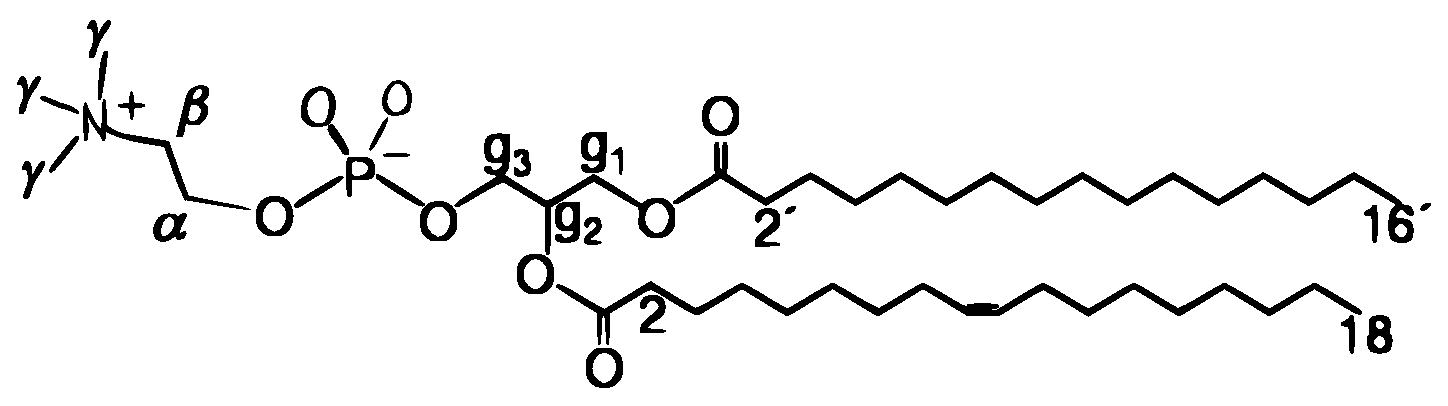
\includegraphics[width=7.5cm]{../Fig/POPCstructure.eps}
  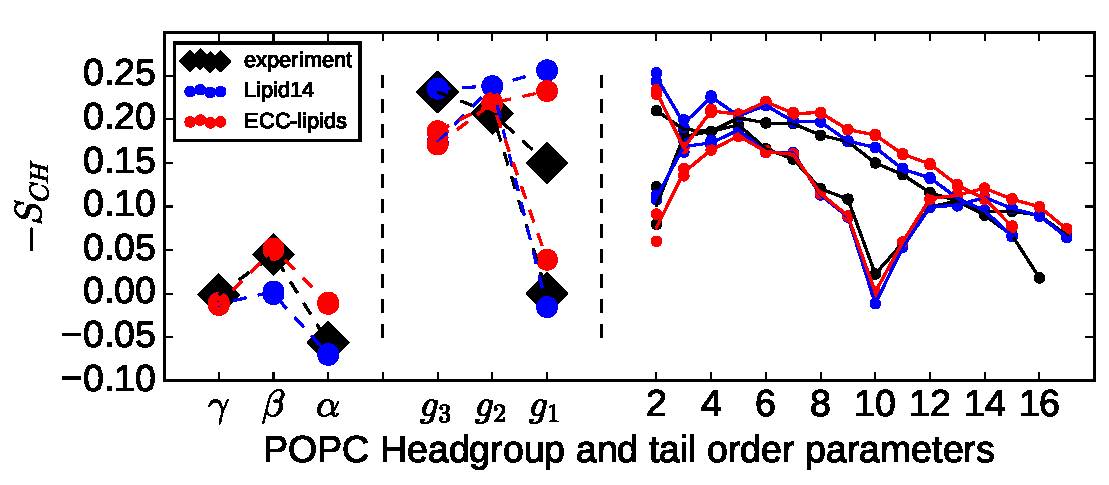
\includegraphics[width=8.0cm]{../Fig/ipython_nb/Order-parameters_exp-L14-ECCL17_q80_sig89.pdf}
  \includegraphics[height=8.4cm,angle=-90]{../Fig/form-f_exp-l14-eccl17.eps}
  \caption{\label{simVSexpNOions}
    Top: Chemical structure of POPC with definitions of different order parameters calculated.
    Middle: Order parameters of head group, glycerol backbone and sn-1 and sn-2 tails  
    from simulations with Lipid14 \cite{dickson14} and ECC-lipids models
    compared with experimental order parameters from \cite{ferreira13}.
    Error bars are approximately the size of the points for head group order parameters.
    Point size for the order parameters of tails are decreased by a factor of 3 to improve the clarity of the plot.
    Bottom: X-ray scattering form factors from experiments~\cite{Kucerka2011} and simulations using Lipid14 \cite{dickson14} and ECC-lipids models. 
    } 
\end{figure}

\begin{table}
  \caption{Area per lipid (APL) from different models of POPC with no ions\label{tab:apls} }
  \begin{tabular}{l|c c}
    model          & APL (\AA$^2$)   & Temperature [K] \\
    \hline
    Lipid14                   & 65.1$\pm$ 0.6  &  300 \\
    Lipid14 \cite{dickson14}  & 65.6$\pm$ 0.5  &  303 \\
    \hline
    ECC-lipids                & 62.2$\pm$ 0.6  &  300       \\
    \hline
    experiment \cite{jambeck12}\todoii{REF}{put original references, not Slipids param. paper.} & 64.3  &  303    \\
    \hline
  \end{tabular}
\end{table}


%In order to validate the structural properties of the newly developed ECC-lipids model
%we first compared our simulation results without any ions to
%NMR order parameters measurements and x-ray scattering form factors 
%(Fig.~\ref{simVSexpNOions}). 
The x-ray scattering form factor (Fig.~\ref{simVSexpNOions}) and
the area per lipid (Table~\ref{tab:apls}) of POPC bilayer simulated
with the ECC-lipid model are in good agreement with the experimental results,
as well as with the Lipid14 model. Thus, we conclude that the lipid bilayer dimensions
are well captured by the developed ECC-lipid model. 
Areas per lipid of ECC-lipids with various other water models are documented in SI, table~\ref{tab:apls_si}. 
%The optimal value for $f_\sigma$ was found by representing the overall membrane structure well
%by matching scattering form factors to experimental data~\cite{Petrache06, Kucerka08, Pabst10}.

As in the original Lipid14 model~\cite{dickson14}, the acyl chain order parameters of the
ECC-lipid model agree well with the experimental values in Fig.~\ref{simVSexpNOions}. Notably, the experimentally measured forking and
small order parameter values of $C_2$ segment in {\it sn}-2 chain are relatively well
reproduced by the both models. This has been suggested to indicate that the carbonyl
region of {\it sn}-2 chain is directed towards the water phase, in contrast to the
carbonyl in {\it sn}-1 chain, which would orient more along the bilayer
plane~\cite{seelig75,schindler75,gawrisch92}. While this may be an important
feature for the ion binding details, it is not necessarily reproduced by the
available lipid models~\cite{ollila16}
%This is expected as the ECC model does not modify
%the already highly optimized parameters of this region in Lipid14. 

The headgroup order parameters of $\alpha$ and $\beta$ carbons are slightly larger
in the ECC-lipid model than in Lipid14, which is apparently related to the
smaller P-N vector angle with respect to the membrane normal in
Fig.~\ref{OrderParameterCHANGESsurf}. With the current data we cannot,
however, conclude which one of the models give the more realistic
headgroup conformations. The ECC-lipid model gives
the $\beta$ carbon order parameter value closer to experiments, while
value for $\alpha$ carbon is better in Lipid14.
Despite of some deviations from the experimental order parameter values
in Fig. \ref{simVSexpNOions},
the accuracy of the both models in the glycerol backbone region
is comparable to the other state
of art lipid models available in literature \cite{botan15}.


\todo{Dynamics check is missing: MSD (Hector/Joe)}

\subsection{Response of POPC head groups to bound charge}

\begin{figure}[tbp]
  \centering
  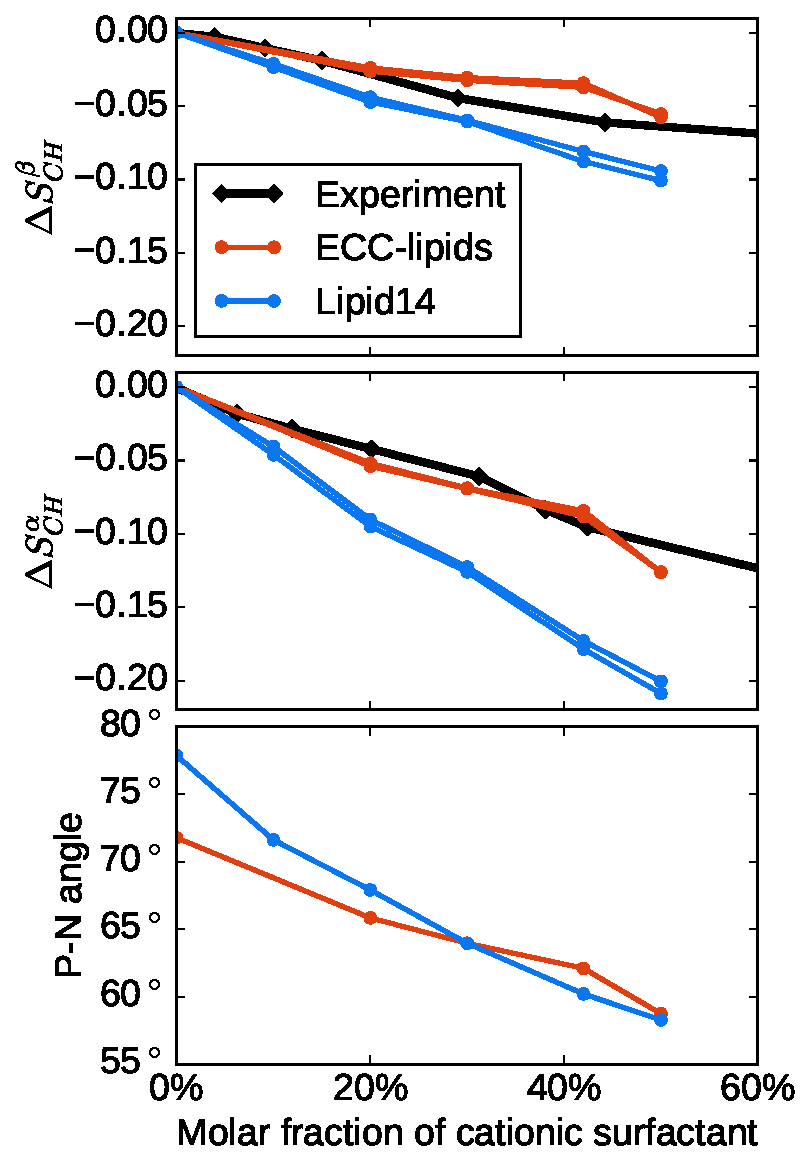
\includegraphics[width=8.0cm]{../Fig/ipython_nb/PN_angle_OrdPars-A-B_L14-ECCL17_q80_sig89_surf.pdf}
  \caption{\label{OrderParameterCHANGESsurf}
    Headgroup order parameter changes and P-N vector orientation as a function of
    cationic surfactant (dihexadecyldimethylammonium bromide, 2C$_{16}$$^+$N2C$_1$Br$^-$)
    in PC bilayer from simulations and experiments \cite{scherer89}.
  }
\end{figure}

Before proceeding to the ion binding affinity, we quantify
the response of headgroup order parameters to the amount of 
bound charge by using mixtures of monovalent cationic surfactants
and POPC~\cite{scherer89}. The amount of bound charge per PC 
in these systems is given by the molar fraction of cationic 
surfactants, because essentially all surfactants locate in the 
lipid bilayers. Experimental data for these systems can be used to validate 
the sensitivity of lipid headgroup order parameters
to the amount of bound charge in simulations.

%depends on both, the
%binding affinity and the response of the head group on bound charge.
%Thus, the head group response to bound charge has to be correctly
%described in the model if the concept is used for quantitative studies of
%binding affinity. Hence, we first quantify the response of head group order
%parameters to the bound charge by using experimental data measured from
%mixtures of cationinc surfactants and PC lipids~\cite{scherer89}.
%
%Thus, the head group order parameter response to bound charge can be first
%quantified aginst experimental data before proceeding to binding affinity studies.
%Headgroup order parameter response to the amount of bound charge can
%be quantified by using ionic surfactants with a known valency~\cite{scherer89}.
%All surfactants locate in lipid bilayers due to their amphiphilic nature,
%thus the exact amount of bound charge in the membrane is known in these systems.
%The head group order parameter changes as a function of bound charges can be then
%explicitly determined from such systems.

The headgroup order parameter changes with an increasing amount of 
the cationic surfactant dihexadecyldimethylammonium bromide 
is compared between experiments~\cite{scherer89} and simulations in
Fig. \ref{OrderParameterCHANGESsurf}. 
The observed order parameter decrease in simulations and experiments
can be approximated to be linear at least for mole fractions
below $\sim$30\%, as expected from Eq. \ref{OPchangeEQ}.
The slope is, however, too steep in the Lipid14 model indicating that 
the head group order parameters are too sensitive to a bound charge.
The ECC-lipids model gives a slope in very good agreement with experiments
for the $\alpha$ segment, while the slope is slightly
underestimated for the $\beta$ segment.
%This has to be taken into account when interpreting the
%head group order parameter response to CaCl$_2$ concentration in Lipid14 model.
%observed in  Ref. \citenum{catte16}, see also Fig. \ref{fig:delta_ordPar_NaCl}.
%The present comparison of head group order parameter changes 
%suggests that the observed overestimated response of all models to 
%increasing CaCl$_2$ concentration in \cite{catte16} 
%can be explained at least in part by a high sensitivity of the head group order parameter response
%to the bound charge.
\todo{SAMULI: We could calculate the slopes from simulations, but I am not sure if
we would actually learn anything useful from this.}

The headgroup P-N vector angle with respect to the membrane normal
is also shown as a function of cationic surfactant mole fraction
in Fig.~\ref{OrderParameterCHANGESsurf}.
The headgroup orients more towards the water phase with an increasing
amount of bound cations, as previously reported in Ref.~\citenum{seelig87}. 
The effect is more pronounced in Lipid14 than 
in ECC-lipids model, which is in line with the order parameter 
results and the reduced charge--dipole interactions in the latter model.
The response of $\alpha$-order parameter to bound positive charge
in ECC-lipid model is in good agreement with experiments.
The model can be thus used to study changes of lipid P-N vector
in varying conditions.

%
%Therefore we use the data in Fig.~\ref{OrderParameterCHANGESsurf}
%to suggest a linear relation between $\alpha$-carbon order parameter
%and average P-N vector angle changes $\Delta \Theta_{\rm P-N}=?? \Delta S_{\rm CH}^{\alpha}$.
%This can be used to estimate the change in P-N vector angle
%from experiments measuring changes in $\alpha$-carbon order parameter. 
%\todo{SAMULI: I think that we should establish the relation between 
%order parameter and P-N vector angle changes by using ECC-lipids model.
%This would be useful for people measuring aplha order parameter
%changes from experiments.}
%
%For example, $\Delta S_{\rm CH}^{\alpha}=0.018$ measured due to the
%addition of 66.8 $\mu$M concentration of Mellittin in bulk water \cite{kuchinka89}
%gives $\Delta \Theta_{\rm P-N} = 2.5^{\circ}$.
%\todo{I looked this roughly from the figure, should be calculated from 
%the actual relation if we decide to put this.}


\subsection{Cation binding affinities to POPC}

\begin{figure}[tbp]
  \centering
  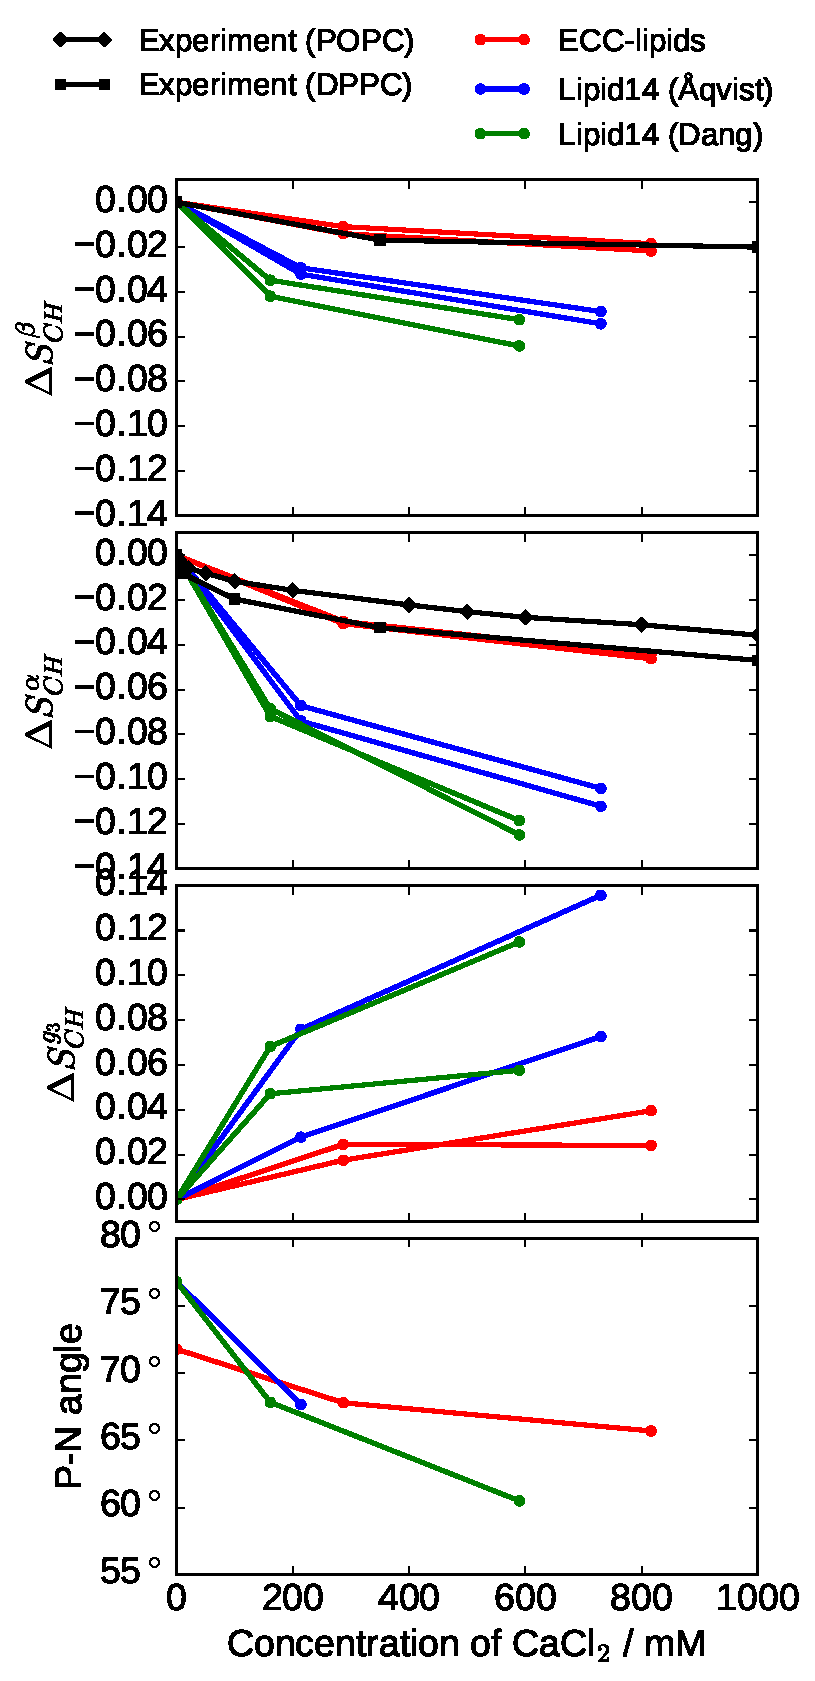
\includegraphics[width=7.5cm]{../Fig/ipython_nb/PN_angle_OrdPars-A-B-g3_L14-ECCL17_q80_sig89_CaCl.pdf}
  \caption{\label{fig:delta_ordPar_CaCl}
    Changes of head group order parameters of POPC bilayer as a function of CaCl$_2$ concentrations
    are shown from simulations with different force fields together with experimental data 
    (DPPC \cite{akutsu81} and POPC \cite{altenbach84}). 
    Ion concentrations in bulk water are shown in x-axis. 
    Values from simulations are calculated from the of cation number density $C_{np}$
    from the region at the simulatin box edge with the constant ion concentration as [ion]=$C_{np}/0.602$.
    Simulation data with Lipid14 and \AA{}qvist ion parameters is taken directly from Ref. \cite{catte16}.
  }
\end{figure}

The binding affinities of aqueous cations to lipid 
bilayers can be measured using the headgroup 
order parameters, because they decrease proportionally  
to the bound positive charge~\cite{seelig87,catte16}. 
The headgroup order parameter responses 
to increasing aqueous CaCl$_2$ concentrations 
from experiments (DPPC \cite{akutsu81} 
and POPC \cite{altenbach84}) and different simulation models for POPC 
are shown in Fig.~\ref{fig:delta_ordPar_CaCl}.
Responses to NaCl concentrations are in SI, Fig.~S\ref{fig:delta_ordPar_NaCl}.

%The simulation results of Lipid14 with \AA{}qvist ions~\cite{aqvist90} (from Ref. \citenum{catte16})
%are shown together with the results from Lipid14 simulation
%with ions by Dang~\cite{smith94,chang1999,dang2006} and from ECC-lipids simulations with ECC-ions.

Negligible changes of the headgroup order parameters are measured
with submolar concentrations of NaCl due to the very low affinity of Na$^+$
in PC bilayers \cite{akutsu81}. While Na$^+$ binding and the related 
headgroup order parameter changes were overestimated in
almost all the available simulation models, the low affinity
and negligible order parameter changes were reproduced by Lipid14 
model when simulated with \AA{}qvist ions~\cite{catte16}.
However, the same combination of force field parameters
overestimated the headgroup order parameter response to CaCl$_2$ 
concentration, which was the case also in all other models tested in
Ref.~\citenum{catte16}.
Using the ion model by Dang et al.~\cite{smith94,chang1999,dang2006} or
ECC-ions~\cite{jungwirth17-new-paper-to-be-published, kohagen16, Pluharova2014}
with more realistic bulk behaviour did not improve the results
for the CaCl$_2$ interactions with a POPC bilayer described by the Lipid14 model, as seen 
in Figs. \ref{fig:delta_ordPar_CaCl} and S\ref{fig:ordPars_waterModels} (in SI), respectively.
\todo{Add OP-response of Lipid14+ECC-ions plot in SI}.
The results support the conclusion of the previous work \cite{catte16}
that improvements also in lipid models are needed to 
correctly describe divalent cation binding to PC bilayers.

Significant improvement can be achieved using the ECC
approach also for lipids. The headgroup order parameters change
as a function of CaCl$_2$ concentration for the ECC-lipid model with ECC-ions
exhibit a good agreement with experiments in Fig.~\ref{fig:delta_ordPar_CaCl} and S\ref{fig:delta_ordPar_NaCl}.
As discussed in previous section, the model gives also
a good agreement with experiments for
the headgroup response to bound charge.
%Thus, the model can used for more detailed analysis of the binding affinity.


The binding affinities are quantified using
the water density profiles along the membrane normal shown
in Fig.~\ref{fig:cacl-dens}. The density profiles show
a larger Ca$^{2+}$ density peak in lipid headgroup region for
the Lipid14 model with Dang and ECC-ions than for the ECC-lipid model.
The relative surface excess calculated from Eq.~\ref{surfexcess} is 
$\Gamma_i^w = 0.07 \pm 0.01 nm^{-2}$ for the ECC-lipid model,
which is significantly smaller than $\Gamma_i^w = 0.13 \pm 0.01 nm^{-2}$ for
Lipid14 with \AA{}qvist and $\Gamma_i^w = 0.3 \pm 0.03 nm^{-2}$ with Dang ions.

\todo{Below analysis is done in a stupid way to get some idea. I would fine it useful to
  do this analysis by using the density profiles, but it is not necessary.
  The reason why I want to do something like this, is that it would be useful to have
  some easier way to estimate the correct binding affinity than the electrometer concept,
  which is quite tedious to apply in practise (simulations with different concenrations,
  cationic surfactant check, etc.). I wuold like to be able to estimate much faster from a
  simulation if the binding affinity is reasonable or not. This may not be the correct way for
that anyway.}
Rough estimates for the free energy difference between bound and unbound cation
are given by
\begin{equation}
  \Delta G = -{\rm k_b T}\log(\frac{p_i}{p_o}),
\end{equation}
where $p_o$ and $p_i$ are estimated from the Ca$^{2+}$densities in bulk water and
in the maximum density in bilayer, respectively. The density profiles in
Fig. \ref{fig:cacl-dens} give $\sim 0.8$ k$_{\rm b}$T for the free energy difference
between bound and unbound Ca$^{2+}$ ions in ECC-lipid model and $\sim 1.4$ k$_{\rm b}$T
in Lipid14 with \AA{}qvist.

\todo{SAMULI: Maybe we should discuss the repeat distances and
  area per molecules measured at \cite{petrache06,pabst07,uhrikova08}
  }




\begin{figure}[tbp]
  \centering
  \includegraphics[width=9.0cm,angle=0]{../Fig/CAdensities2.eps}
  \caption{\label{fig:cacl-dens}
    Number density of \ce{Ca^{2+}} and \ce{Cl^-} as a function of membrane normal axis
    for different force fields. Data for Lipid14 with \AA{}qvist ions are taken directly from Ref. \citenum{catte16}.
    %Normalization factor for ions is 1 for monovalent ions (i.e.~\ce{Na^+} and~\ce{Cl^-}),
    Densities of~\ce{Cl^-} and water are divided with 2 and 200, respectively, to visalize them
    with the same scale as \ce{Ca^{2+}}. The molar concentration of the ions in water is 350~mM in all systems
    presented here. 
    }
  \todo{PAVEL: draw phosphate position with its variance, add water density (scaled) and include the number of$\Gamma$-surface access.} \\
  \todo{JOE: Change the figure so that it contains a membrane background} \\
\end{figure}

Since the lipid headgroup order parameter responds to the amount of bound charge
and to the aqueous ion concentrations are both in good agreement with experiments
in the ECC-lipid model with ECC-ion parameters, we consider the Na$^+$ and Ca$^{2+}$
binding affinities to be realisticlly described in this model. In contrast, the Ca$^{2+}$
binding affinity is overestimated by Lipid14 model when simulated with all the
tested ion models. Similar conclusions were previously made based only on the headrogup
order parameter data with aqueous cations~\cite{catte16}. However,
the discrepancies with experiments in previous work could partly arise also from
the inaccurately described sensitivity of the headgroup to bound charge. Here we quantify this
effect and conclude that the improvement due to ECC is to a large extent, but not entirely,
caused by a more realistic headgroup sensitivity to bound charge.
This indicates that the issue should be carefully considered also when
the electrometer concept is used to compare ion binding between experiments
and simulations with other models.


%The good agreement with experiments indicates
%that the ECC corrected lipid model has a sufficient accuracy for realistic
%studies of details of ions binding to lipid bilayers.



\subsection{Binding stoichiometry}

%Binding probability:
%\ce{Ca2+} complex with \\
%1 POPC - 13\% -- 30\% \\
%2 POPC - 18\% -- 42\% \\
%3 POPC - 12\% -- 28\% \\

This section is rough and will likely require editing. 
Data -- up to noted exceptions -- shall be all there, however. 
\todo{SAMULI: I think the we should make clear that the current binding
  constants in, e.g., Marsh's handbook are based on the headgroup order parameter
  changes intepreted with ternary complex binding model. I.e. the experimental raw data
  is excatly the same as we have in this work. Our simulations enable much more versatile interpretation
  of the binding phenomena. I think that this is one the main points of this work, so this comment
  applies to the previous section, introduction, abstract and conclusions as well.
}

Binding stoichiometry of \ce{Ca^{2+}} and POPC was 
thoroughly studied in the experimental work~\cite{altenbach84},
in which the head group order parameter changes to cation binding are determined.
Several binding models were proposed and tested of which only one,
ternary complex binding model, provided a good fit of the experimental observations. 

Simulations allow us to directly evaluate the stoichiometry 
by calculating relative propensities of various \ce{Ca^{2+}}:$n\times$POPC clusters
by evaluating contacts between cations and lipids with a cut off radius $0.3\,\mathrm{nm}$. 
In Figure~\ref{fig:cacl_complexes} we see that ternary complex is indeed 
the most probable binding mode of calcium at 285~mM concentration. 
Apart from this complex, we also find complexes with 1~and 3~lipids
occuring with only a slightly lower but similar probability.
The fractions of \ce{Ca^{2+}}:$n\times$POPC complexes at 285~mM concetration 
are then in order:
$42\%$ for two lipids,
$30\%$ for one lipid, and
$28\%$ for three lipids.

Several binding models were proposed and tested~\cite{altenbach84} of which only one,
ternary complex binding model, provided a good fit of the experimental observations. 
In such a model, it is assumed that \ce{Ca^{2+}} cations bind to a POPC membrane 
with a stoichiometry 2~POPC:1~\ce{Ca^{2+}}.
In a later work~\cite{macdonald87}, 
a Langmuir adsorption model (i.e. stoichiometry 1~POPC:1~\ce{Ca^{2+}}) 
was found to provide as good fit as ternary complex model, 
when only low concentrations of \ce{CaCl2} are considered.
Ternary complex model also provides a good fit 
to our simulations with ECC-lipids 
(see Fig.~\ref{fig:cacl-bind} in SI and its caption for details). 
The symmetry of the distribution of complexes from simulation --  
i.e. almost equal probabilities of complexes with 1 or 3 lipids 
that behave in the total average picture as complexes with 2 lipids -- 
provides clues why ternary complex binding model 
fits both simulation and experimental results relatively well, 
although it is apparently incorrect. 

\begin{figure}[tbp]
  \centering
  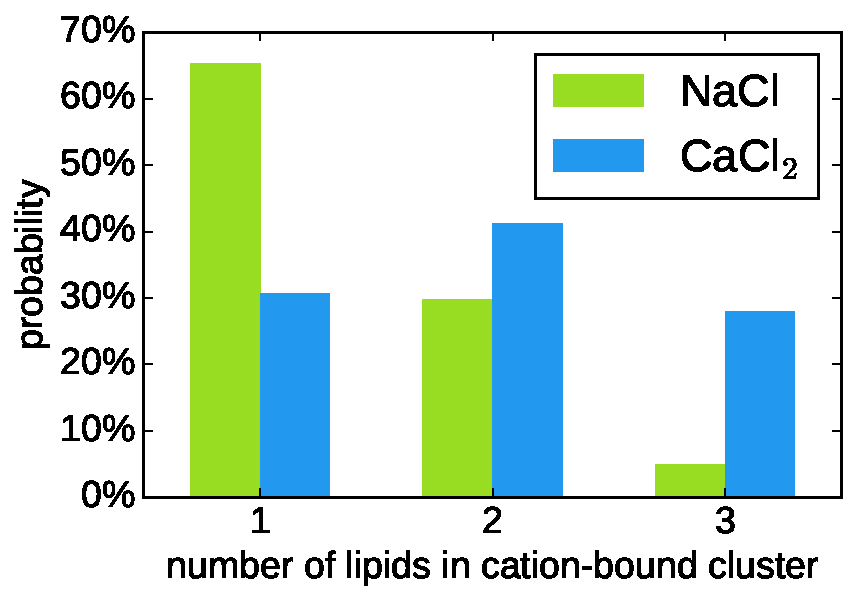
\includegraphics[width=6.0cm]{../Fig/ipython_nb/stoichiometry_NaCl-CaCl2_comparison_Ecc-lipids.pdf} \\
  \caption{\label{fig:cacl_complexes}
      Relative probabilities of existence of \ce{Na^{+}} or \ce{Ca^{2+}} complexes
      with a certain number of POPC lipids. 
      \ce{Na^{+}} complexes were evaluated from the simulation with 1~M concentration;
      and \ce{Ca^{2+}} complexes were evaluated from the simulation with 287~mM concentration.
  }
\end{figure}

In addition, we estimated relative binding affinities 
of several moieties in POPC towards \ce{Ca^{2+}}. 
The dominant contribution
to the binding of \ce{Ca^{2+}} to POPC membranes comes from the phosphate group. 
Such a finding is supported by the calculated
number of contacts between \ce{Ca^{2+}} and POPC oxygen atoms.
The average number of contacts between \ce{Ca^{2+}} and any oxygen atom in POPC is 59.8, 
whereas if only phosphate oxygen atoms are considered 
the average number of contacts decreases only by a tiny amount to 57.2. 
We corroborate this finding with the probability isodensity contours in Fig.~\ref{fig:volmaps}, 
which are easier to interpret.

The residence time of \ce{Ca^{2+}} bound to a POPC membrane 
is experimentally estimated to be lower than $10\,\mu\mathrm{s}$~\cite{altenbach84}. 
From recent theoretical work with long enough simulations this time can be roughly estimated
in the order of $1$--$10\,\mu\mathrm{s}$~\cite{javanainen17}. 
This is in contrast to our model, ECC-lipids, 
which gives a mean residence time in the order of $10\,\mathrm{ns}$, 
\todo{evaluate this number, mean residence time, accurately based on the contacts data.}
i.e. at least two orders of magnitude lower than previous estimates.
Such a finding changes the point of view of calcium binding from
very tight long-term stable binding with rare exchanges to 
a relatively frequent exchange of cations 
in equilibrium between membrane and solvent. 


\todo{Finalize stoichiometry analysis for \ce{Na^+}, \ce{Ca^{2+}},
  their interaction energies with the lipid membrane, etc,
  and finalize the discussion after these results.}

%It is also suggested that the addition of \ce{NaCl} to the solution of \ce{CaCl_2} enhances the hedgroup 
%order parameter response compared to the solution with only \ce{CaCl_2}. \cite{altenbach84}
%\todo{Simulate this effect and discuss it further}

%\todo{The difference between DPPC and POPC -- simulate and compare with experiment. }


%\todo{It might be worth acknowledging each experimental finding in \cite{Altenbach84} and observations in \cite{Javanainen2017-ChemComm}.}


\begin{figure}[tbp]
  \centering
  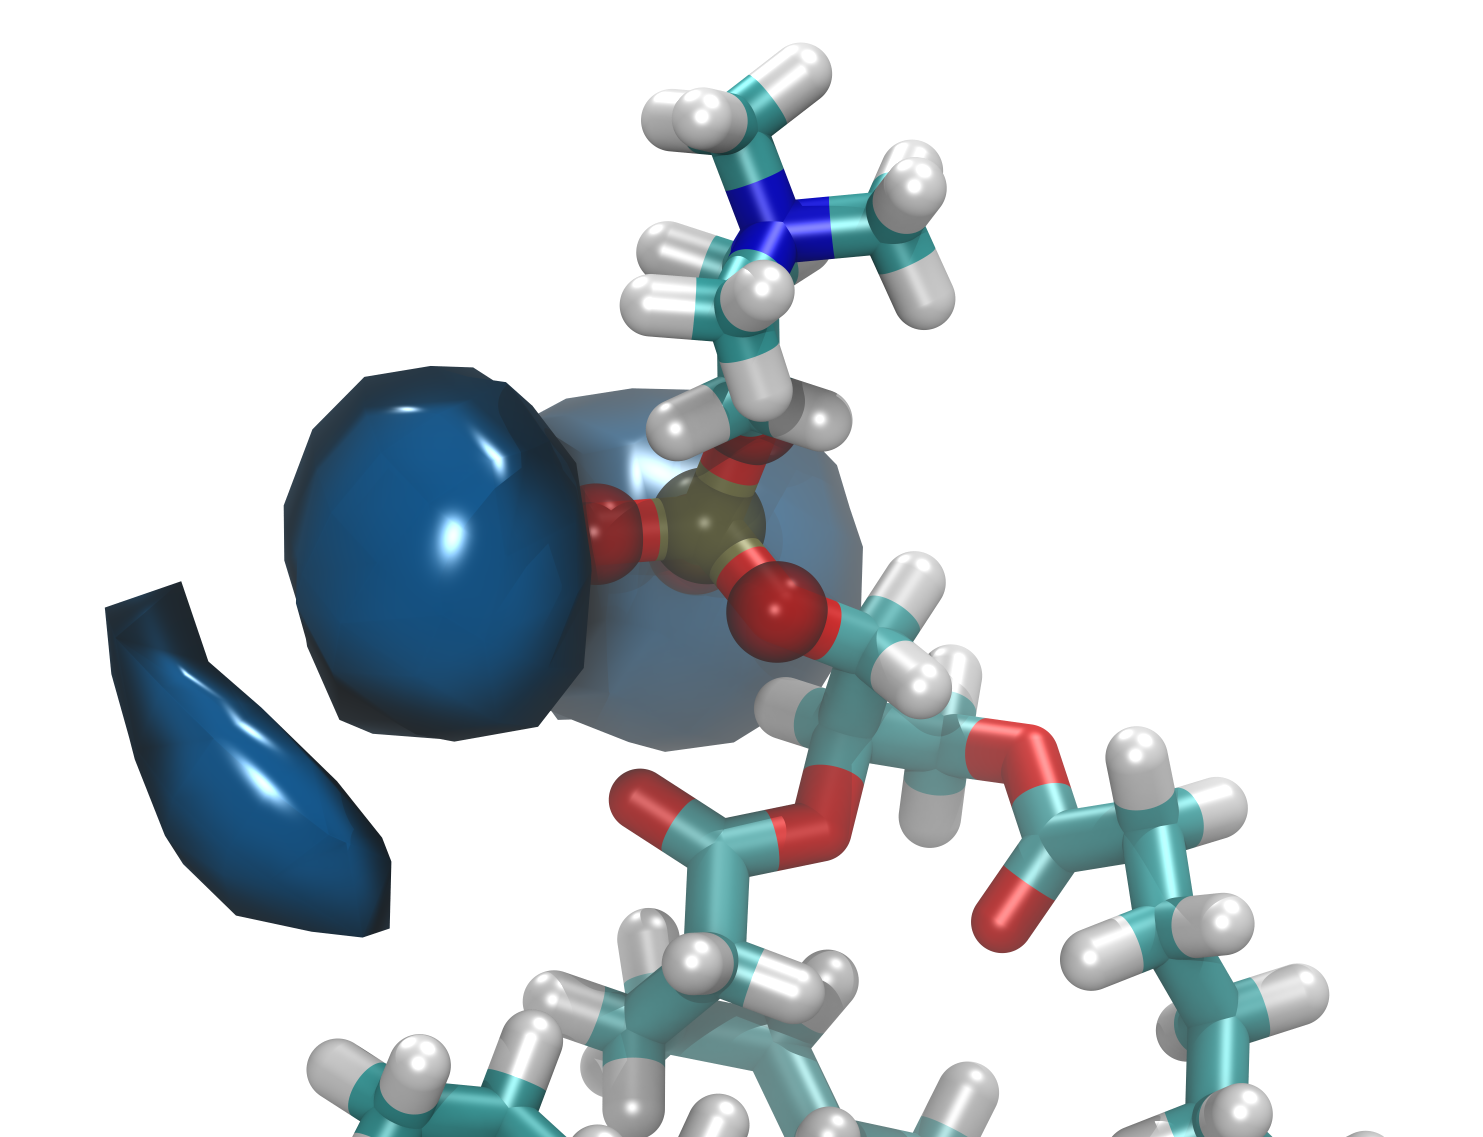
\includegraphics[width=6.0cm]{../Fig/volmap_resid10_Ca_Cl_PO4Cent.png} \\
  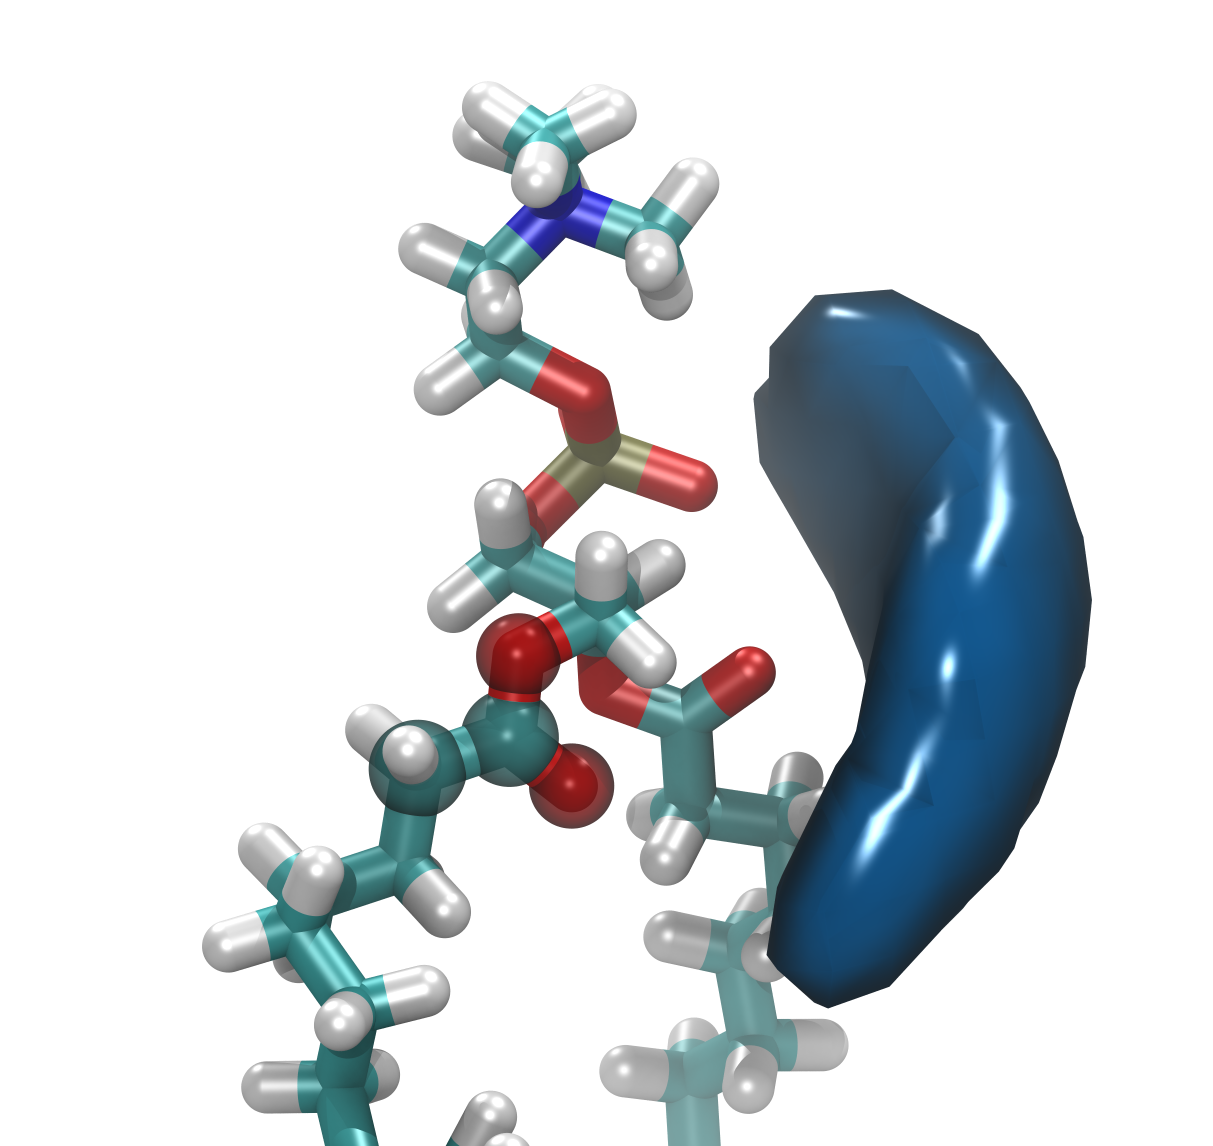
\includegraphics[width=4.0cm]{../Fig/volmap_resid10_Ca_Cl_sn1Cent.png}
  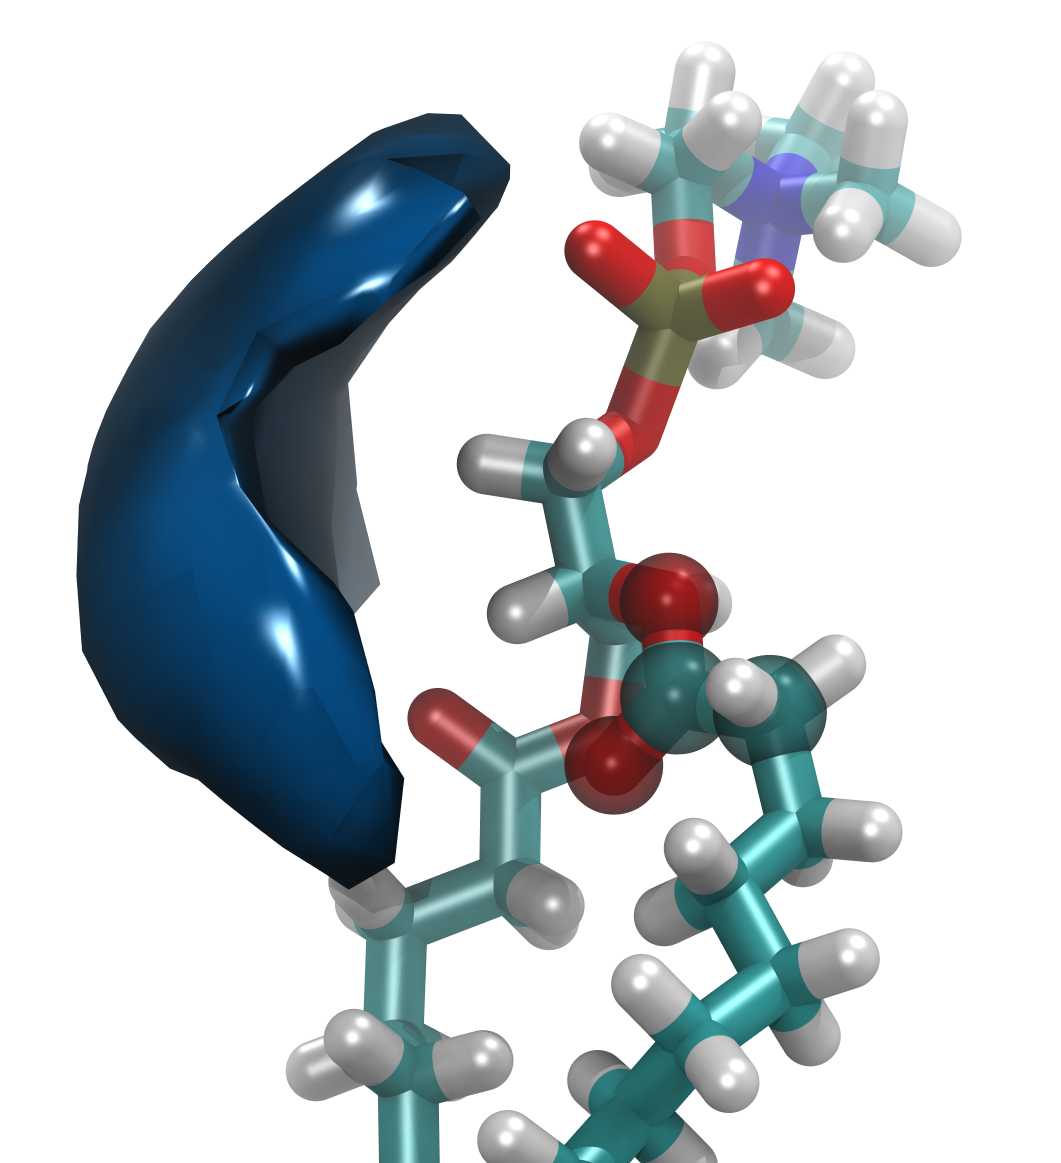
\includegraphics[width=3.6cm]{../Fig/volmap_resid10_Ca_Cl_sn2Cent.png}
  \caption{\label{fig:volmaps}
      Contours of probability isodensities of \ce{Ca^{2+}} with respect to 
      various moieties fixed in space (highlighted with transparent spheres): 
      phosphate moiety, side chain 1 carbonyl group and side chain 2 carbonyl group.
      Shown contours suggest that the dominant contribution 
      to \ce{Ca^{2+}} binding comes from the phosphate oxygens,
      whereas the interactions with any of the two carbonyl groups are considerably milder.
  }
  \todo{JOE: I'll update this figure with some ensemble of configuration to support binding preference of \ce{Ca^{2+}}}
\end{figure}


%\begin{figure}[tbp]
%  \centering
%  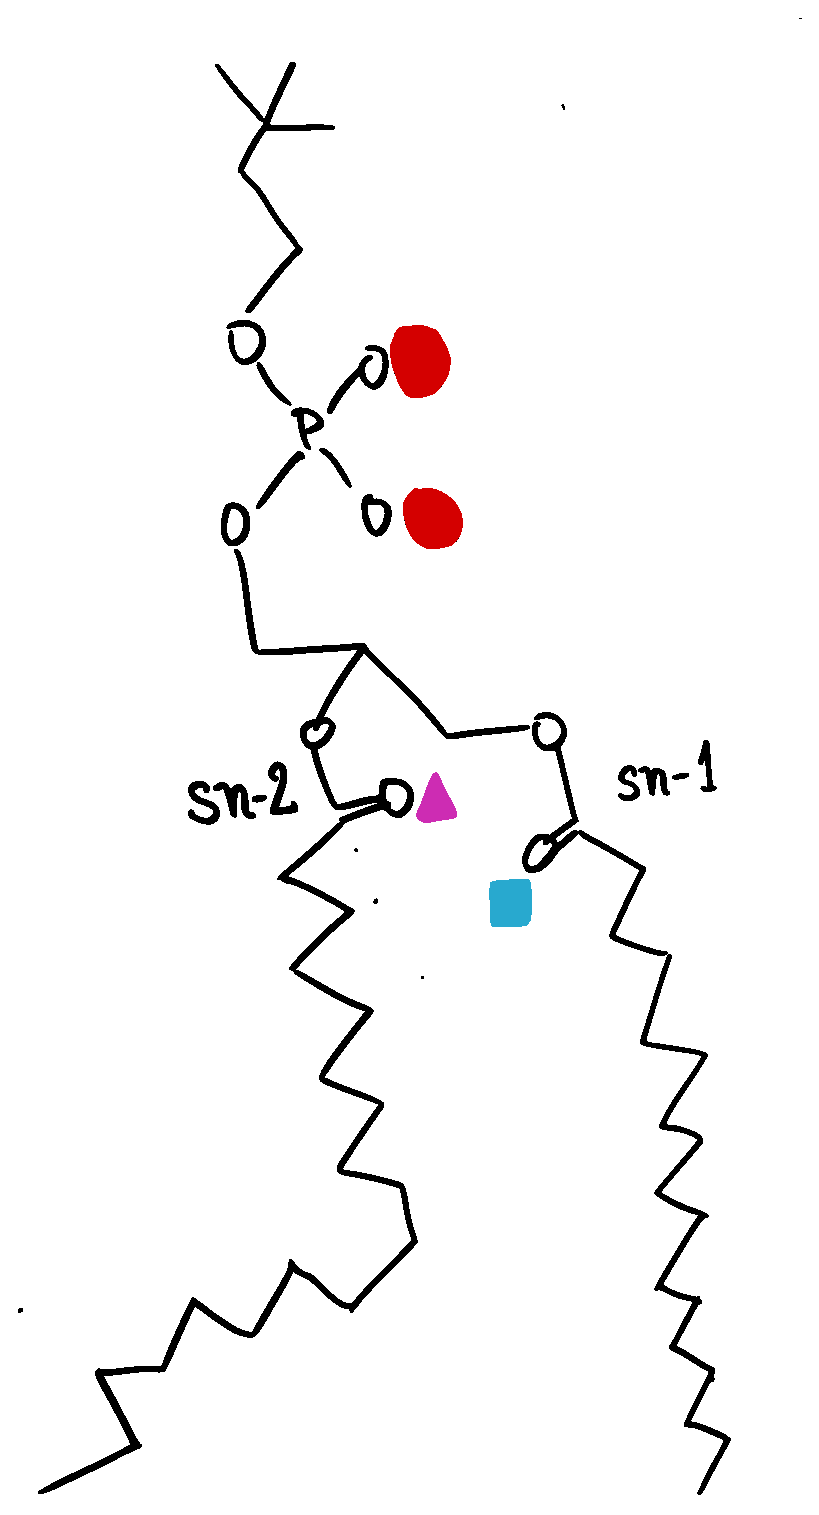
\includegraphics[height=6.0cm]{../Fig/POPC_binding_labels.eps} 
%  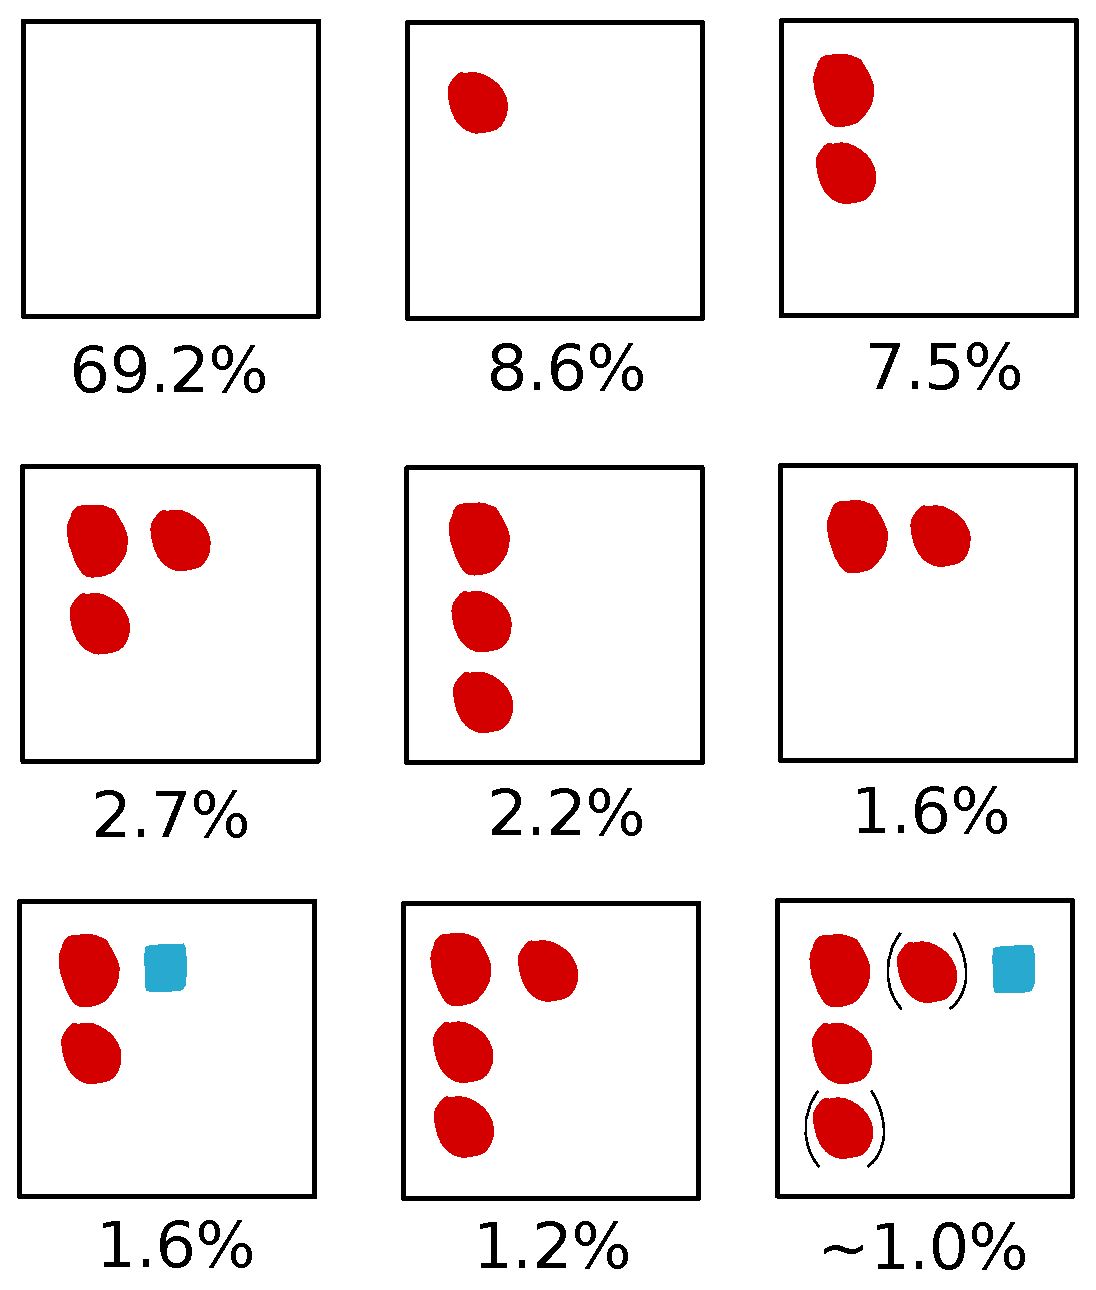
\includegraphics[height=6.0cm]{../Fig/POPC_binding_ECC-lipids.eps}
%  \caption{\label{fig:binding_conf}
%      Configurations of \ce{Ca^{2+}} binding in POPC membranes in the ECC-lipids model.
%      The binding sites are: 
%      red circle for phosphate oxygens; 
%      blue square for sn-1 carbony oxygen; and green triangle for sn-2 carbonyl oxygen.
%      The configurations along with their probabilities are drawn in the following manner:
%      each row corresponds to an individual lipid the cation is bound to;
%      symbols denote the site the cations is bound to the respective lipid.
%      An empty configuration denotes an unbound cation in a solvent. 
%  }
%\end{figure}


\section{Conclusions}
By using the electrometer concept we show that the binding of \ce{Na^+} and \ce{Ca^2+} ions
to a POPC lipid bilayer can be accurately described with the classical MD simulation 
force field, where the electronic polarization is implicitly included using 
the electronic continuum correction (ECC)~\cite{leontyev11}.
The proposed ECC-lipids model is a significant improvement over 
other available lipid models, which all overestimate specific cation binding affinities~\cite{catte16}.  
While the structural details of a POPC lipid bilayer simulated with the ECC-lipids
model agree with experiments with the comparable accuracy to the other state of the art lipid models,
it also reproduces the experimental lipid head group order parameter responses to
the cationic surfactant, NaCl and CaCl$_2$ concentrations. 

The good agreement with experiments enables the atomic resolution 
interpretation of NMR experiments by using MD simulations.
In agreement with previous interpretations of experimental data \cite{hauser76,hauser78,herbette84,binder02},
the Ca$^{2+}$ ions mainly interact with phosphate oxygens.
However, the stoichiometry of the binding is significantly more complicated 
than in the previous interpretation of the NMR data based on 
the ternary complex model, where one calcium binds to two POPC molecules~\cite{altenbach84}.
The complexes of one calcium bound to two lipids are the most probable also in the
ECC-lipids model, but the complexes of one or three lipids per one calcium
were observed to be almost equally likely. While the success of the ternary
compex model is understandable based on the simulation results,
a simple binding model cannot detec the complex binding
oberved in the simulation.

The improved cation binding behaviour to POPC bilayer pave the way for
simulations of complex biochemical systems with correctly described
electrostatic interactions in the vicinity of cellular membranes.
The ECC-lipids model is build by scaling the partial charges and
the LJ-radius of the headgroup, glycerol backbone and carbonyl atoms of
the Lipid14 POPC model~\cite{dickson14}. While the Lipid14 model
is compatible with the AMBER force field family, the compatibility of
the ECC-lipids model may be compromised due to the changes in intermolecular
interactions of the scaled atoms. On the other hand, a fully consistent
ECC-force field should include the correction also in other than lipid
molecules, including water. The work toward this direction and the extension
to other lipid molecules and force fields is left for the future studies.

%but we expect that the correction can be used also for other lipids
%and force fields.

%We suggest using state of the art water models like OPC3\cite{Izadi16} or OPC \cite{Izadi14},
%which yield higher accuracy than the traditional TIP3p water model~\cite{jorgensen83}.
%Several water models 
%(OPC3\cite{Izadi16}, OPC \cite{Izadi14}, SPC/E \cite{Berendsen1987} and TIP4p/2005 \cite{Abascal2005}) 
%were used to exemplify the transferability of 
%the parameters of the new ECC-lipids force field. 



This work can be reached as a repository containing all data at \url{zenodo.org:\dots\dots\dots} and as project \mbox{NMRlipids~VI} in \url{nmrlipids.blogspot.fi}.



% If you have acknowledgments, this puts in the proper section head.
\begin{acknowledgments}
% Put your acknowledgments here.
P.J. acknowledges support from the Czech Science Foundation (grant no. 16-01074S) 
and 600 from the Academy of Finland via the FiDiPro award.
\end{acknowledgments}


\newpage
\newpage
\appendix


\begin{center}
{\bf SUPPLEMENTARY INFORMATION}
\end{center}

It was found in the original work~\cite{altenbach84} that 
a ternary complex binding model (i.e.~2~POPC:1~\ce{Ca^{2+}})
provides the best fit to experimental measurements of all considered models in that study. 
In such a model, there is a linear relationship between quantities 
$C_b$, mole fraction of bound \ce{Ca^{2+}} per POPC, and $\sqrt{C_b/C_I}$, 
where $C_I$ is the concentration of free cations at the plane of ion binding~\cite{altenbach84}.
The concentration $C_b$ was obtained from an extrapolation of linear relation 
between deuterium NMR measurements and atomic absorption spectroscopy for low concetrations of \ce{CaCl2}.
Such an extrapolation is valid as long as the mode of \ce{Ca^{2+}} binding 
remains constant throughout the extrapolation range. 
The concentration $C_I$ is determined by using the surface potential by using the Boltzmann equation.
However, Boltzmann theory yields inaccurate results
for divalent cations like \ce{Ca^{2+}}~\cite{Andelman1995}. 
An atomistic simulation, on the other hand, provides these quantities directly without severe assumptions.
\todo{Did you really calculate the $C_I$ from simulations without severe assumptions?
Note that this conctration at the plane of biding, which do not equal the concentration of free cations.}
Hence we hypothesise that the discrepancy between the results in the experiment~\cite{altenbach84} and 
our simulations likely lays in the fact that 
the assumptions and relations used for determinig concentrations $C_b$ and $C_I$ in the experiment~\cite{altenbach84}
gradually do not hold for higher concentrations of \ce{Ca^{2+}}. 


\begin{figure}[tbp]
  \centering
  \includegraphics[height=9.0cm,angle=-90]{../Fig/bound-CAs_conc-eccl17.eps}
  \caption{\label{fig:cacl-bind}
    Ternary complex binding model of \ce{Ca^{2+}} to a POPC membrane 
    that assumes the stoichiometry of 2~POPC:1~\ce{Ca^{2+}} (details in reference~\citenum{altenbach84}) 
    provides a good fit to experimental measurements~\cite{altenbach84}
    and it also provides a good fit to our simulation data. 
    Note that the units in the reference~\citenum{altenbach84} are different from the units presented here,
    and, hence, the observed slope of the linear relationship is different.
    }
\end{figure}


\begin{figure}[tbp]
  \centering
  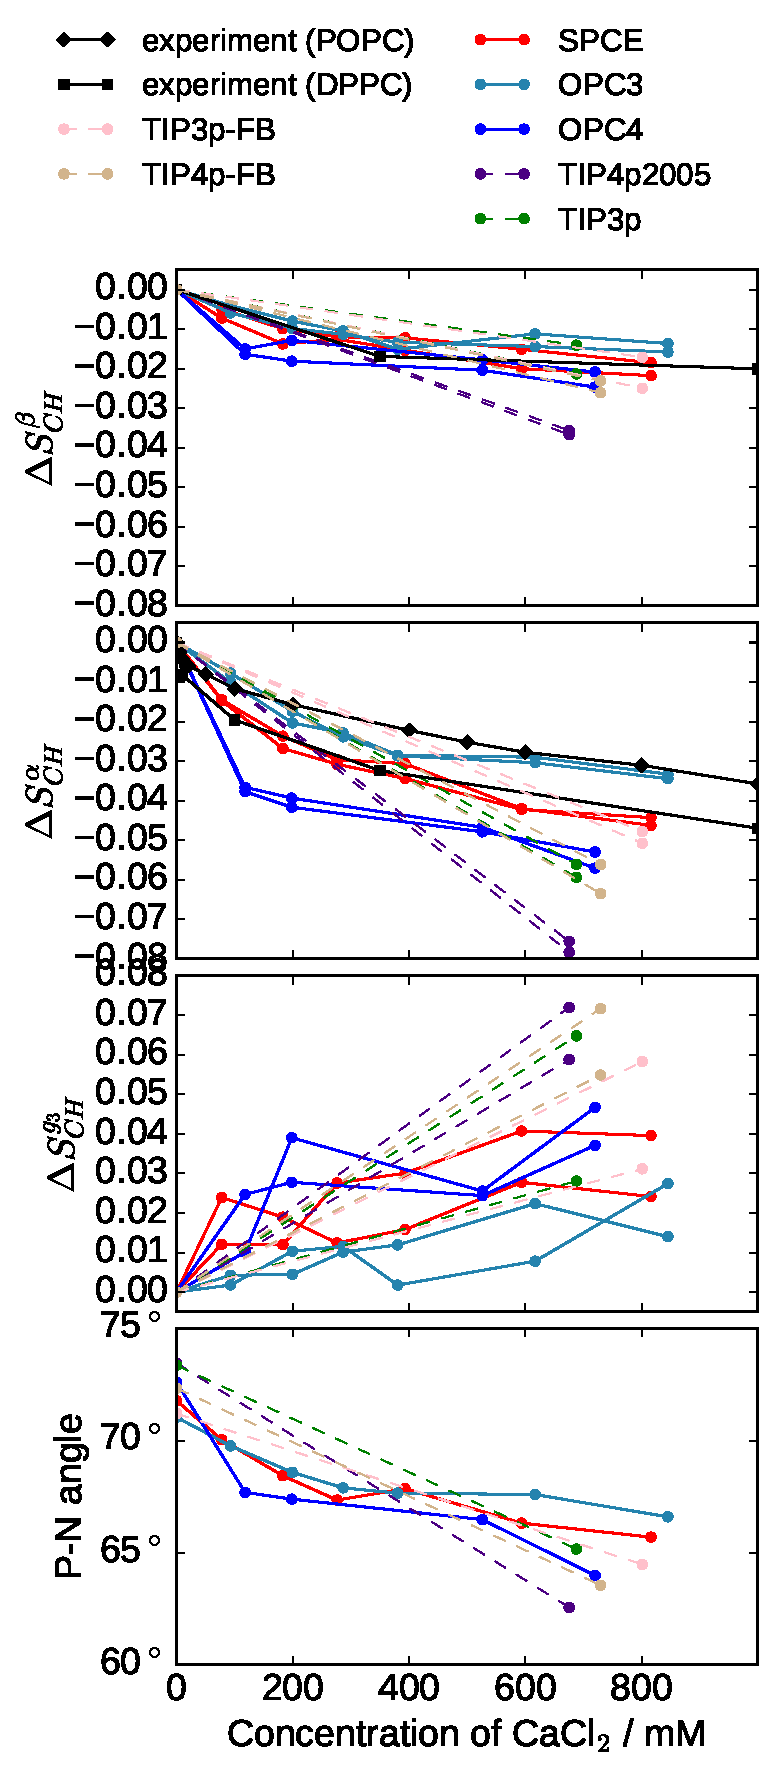
\includegraphics[width=8.0cm]{../Fig/ipython_nb/PN_angle_OrdPars-A-B-g3_L14-ECCL17_q80_sig89_CaCl_waterModels.pdf}
  \caption{\label{fig:ordPars_waterModels}
    Changes of head group order parameters of POPC bilayer as a function of CaCl$_2$ concentrations
    are shown from simulations with different force fields and water models together with experimental data 
    (DPPC \cite{akutsu81} and POPC \cite{altenbach84}). 
    Ion concentrations in bulk water are shown in x-axis. 
    Values from simulations are calculated from the of cation number density $C_{np}$
    from the region at the simulatin box edge with the constant ion concentration as [ion]=$C_{np}/0.602$.
  }
\end{figure}


\begin{figure}[tbp]
  \centering
  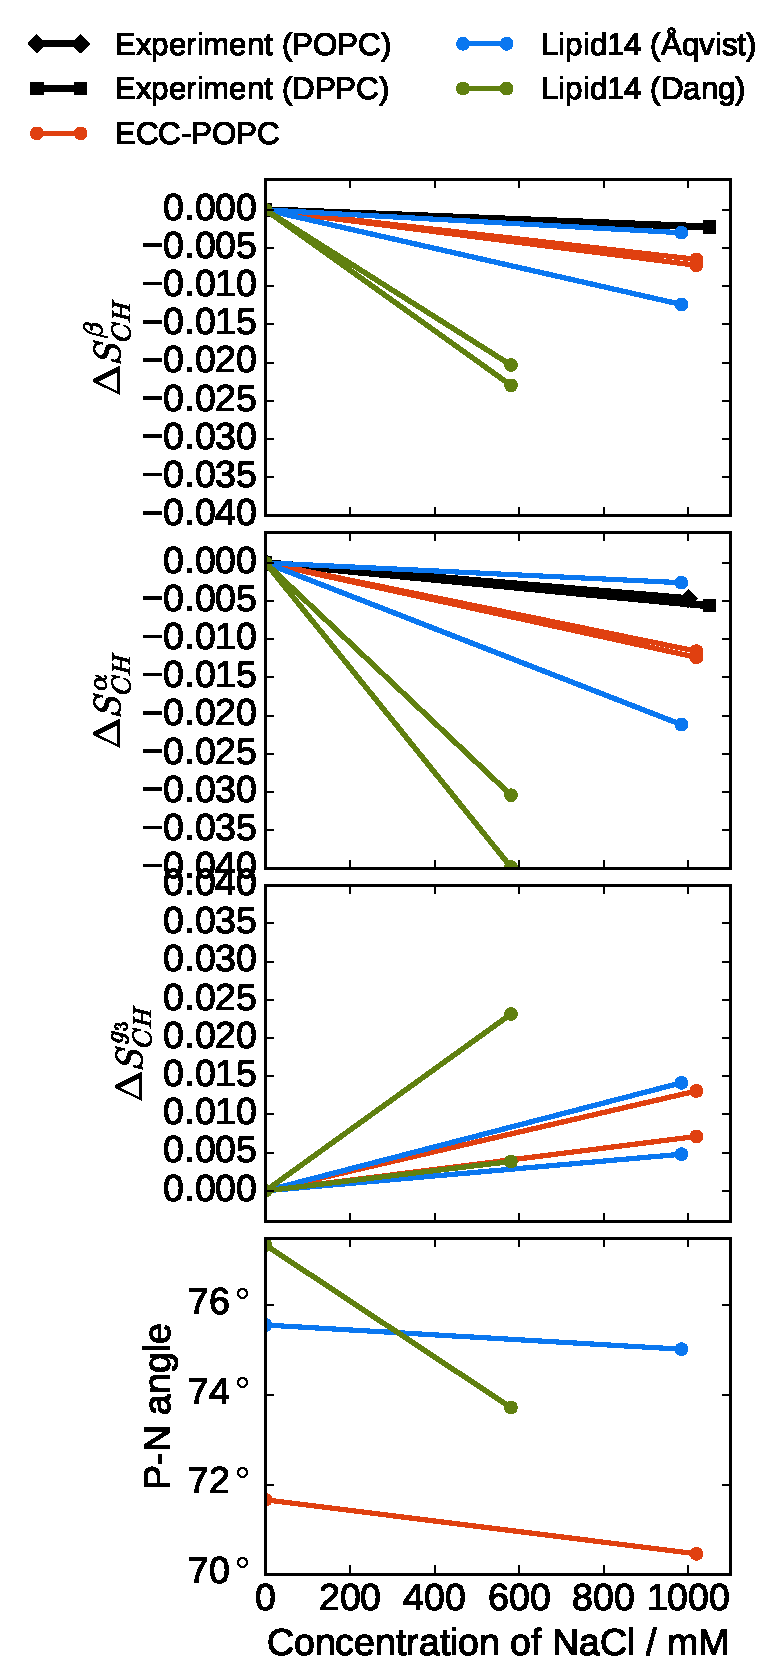
\includegraphics[width=8.0cm]{../Fig/ipython_nb/PN_angle_OrdPars-A-B-g3_L14-ECCL17_q80_sig89_NaCl.pdf}
  \caption{\label{fig:delta_ordPar_NaCl}
    Changes of head group order parameters of POPC bilayer as a function of NaCl concentrations
    are shown from simulations with different force fields together with experimental data \cite{akutsu81}. 
    Ion concentrations in bulk water are shown in x-axis. 
    Values from simulations are calculated from the of cation number density $C_{np}$
    from the region at the simulatin box edge with the constant ion concentration as [ion]=$C_{np}/0.602$.
    Simulation data with Lipid14 and \AA{}qvist ion parameters is taken directly from Ref. \cite{catte16}.
  }
\end{figure}


\begin{table}
  \caption{Area per lipid (APL) from different models of POPC with no ions\label{tab:apls_si} }
  \begin{tabular}{l|c c}
    model          & APL (\AA$^2$)   & Temperature [K] \\
    \hline
    Lipid14                   & 65.1$\pm$ 0.6  &  300 \\
    Lipid14 \cite{dickson14}  & 65.6$\pm$ 0.5  &  303 \\
    \hline
    ECC-lipids &        &  \\
    %Lipid14ecc0.80+sigma0.875 &        &  313    \\
    %($4.6\cdot 5.1 \, \mathrm{nm}^2$), 72 lipids patch, OPC3           & 63.2   &   313      \\
    ~ OPC3           & 62.2$\pm$ 0.6   &  300       \\
    ~ OPC3           & 64.2$\pm$ 0.6   &  313       \\
    ~ SPC/E          & 65.1$\pm$ 0.6   &  313       \\
    ~ OPC            & 64.4$\pm$ 0.6   &  313       \\
    ~ TIP4p/2005     & 66.8$\pm$ 0.6   &  313       \\
    %($9.2\cdot 10.2 \, \mathrm{nm}^2$), 288 lipids patch           & 65.5   &  313       \\ %% not done for this model with f_sigma=0.89
    %oMM small patch           & 63.65  &         \\
    %oMM 4xbig patch           & 63.7   &         \\
    \hline
    experiment   & 62.7  &  293    \\
    experiment \cite{jambeck12}\todoii{REF}{put original references, not Slipids param. paper.} & 64.3  &  303    \\
    experiment  & 67.3  &  323    \\
    experiment  & 68.1  &  333    \\
    %experiment POPE  & 56.6 &  303    \\
    \hline
  \end{tabular}
\end{table}


\begin{table}[btp]
  \caption{Simulation parameters}
  \label{tbl:mdpar}
  \begin{tabular}{ll}
    simulation property & parameter   \\
    \hline
    time-step           & 2~fs         \\
    equilibration time  & 100~ns  \\
    simulation time     & 200~ns  \\
    temperature         & 313~K       \\
    thermostat          & v-rescale  \cite{bussi07}   \\
    barostat            & Parrinello-Rahman, semi-isotropic \cite{parrinello81} \\
    long-range electrostatics & PME  \cite{darden93}  \\
    cut-off scheme      & Verlet \cite{Pall13}      \\
    Coulomb and VdW cut-off & 1.0~nm \\
    constraints         & LINCS, only hydrogen atoms \cite{hess97} \\
    constraints for water & SETTLE  \cite{miyamoto92} \\
    \hline
  \end{tabular}
\end{table}



% Create the reference section using BibTe
\bibliography{refs.bib}

%\newpage
%\section{APPENDIX: The NMR results reported by Tiago Ferreira}

\listoftodos

\end{document}
%
% ****** End of file aiptemplate.tex ******
